\documentclass[12pt]{article}

%packages
\usepackage{graphicx}
\usepackage{amsmath}
\usepackage{mathdots}
\usepackage{amsthm}
\usepackage{amssymb}
\usepackage{fancyhdr}
\usepackage{pstricks}
\usepackage{pst-node}
\pagenumbering{arabic}
\usepackage{hyperref}
\usepackage{lscape}
%Margins etc...
\setlength{\textheight}{240mm}
\setlength{\topmargin}{-17mm} \setlength{\oddsidemargin}{-4mm}
\setlength{\textwidth}{166mm} \setlength{\parindent}{0mm}
\setlength{\marginparsep}{9mm} \setlength{\parskip}{3mm}

\begin{document}
\begin{center}
\Huge{Markov Chains Role Playing Game}\\
\tiny{Last updated: \today.}
\end{center}

This exercise serves as an introduction to Markov Chains:
\begin{itemize}
\item Explain that there are 3 locations (1,2 and 3).
\item Explain that students are going to move between the locations according to the following diagram:
\begin{center}
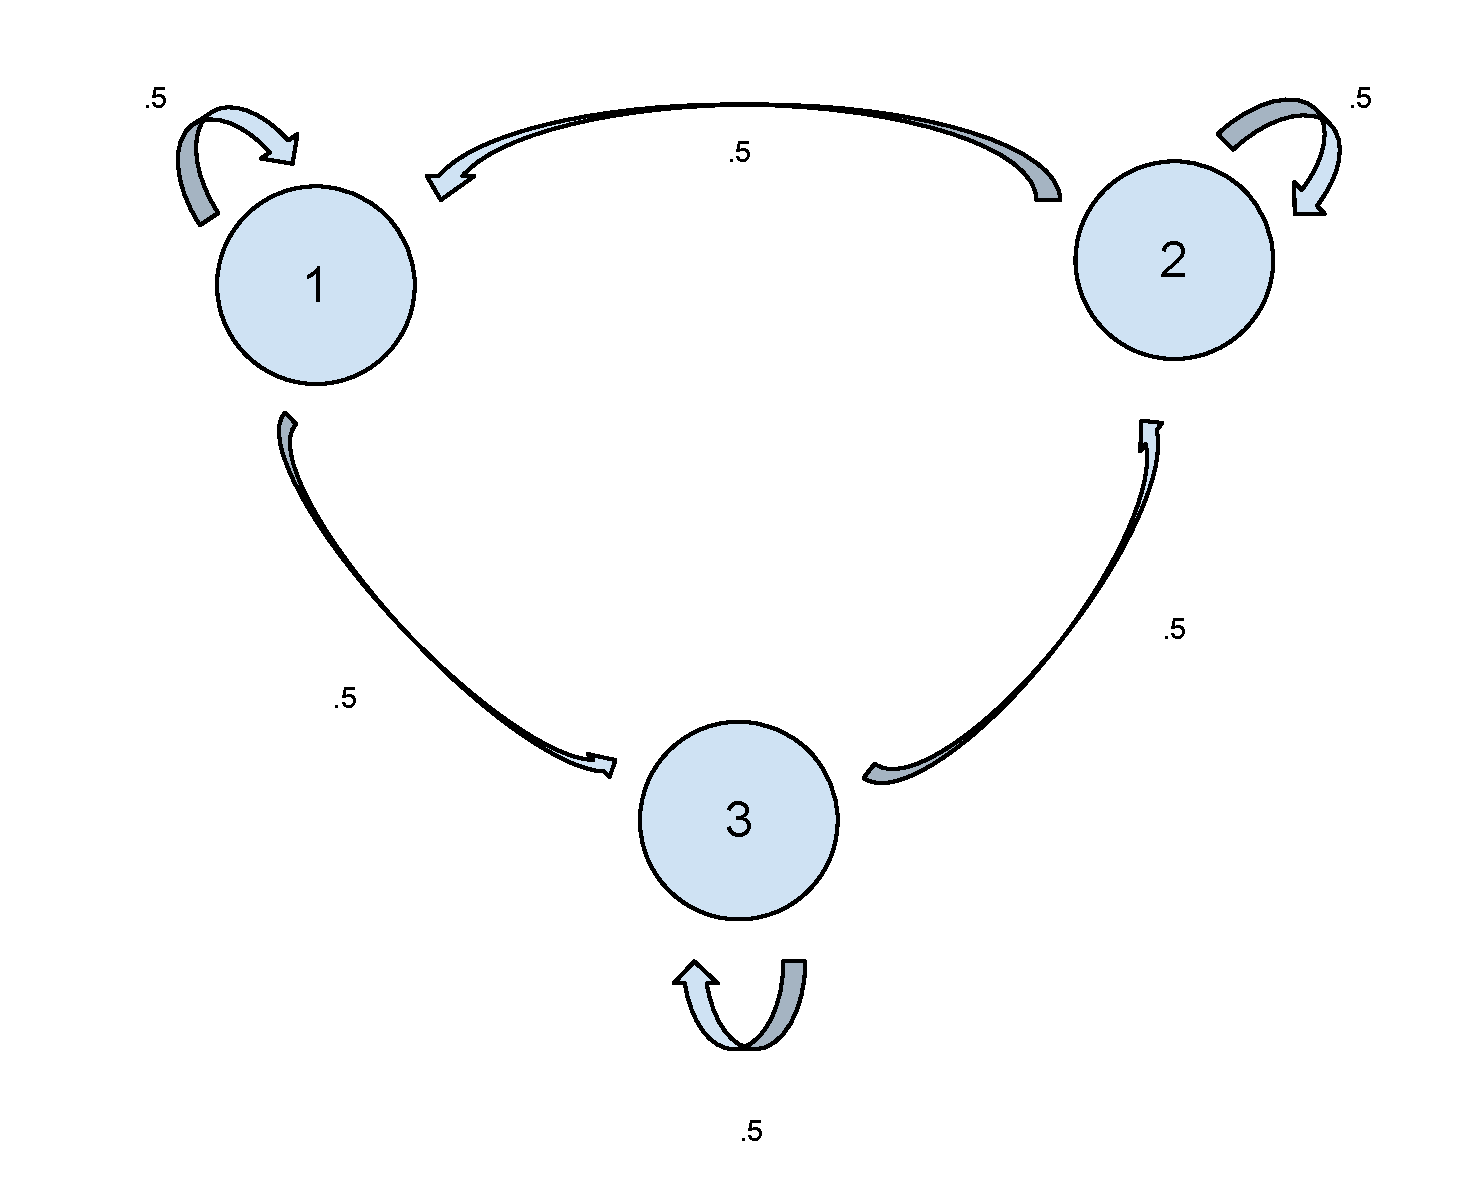
\includegraphics[width=6cm]{role_playing_game.pdf}
\end{center}
\item Explain that in case of a non integer quantity to round up the number of people leaving a location.
\end{itemize}

Use the following two initial set ups which require 12 students and there's no harm in having 1 student to log transitions.

\begin{enumerate}
\item $\pi^{(0)}=(12,0,0)$
\item $\pi^{(0)}=(7,3,2)$
\end{enumerate}

This is the "solution":

\begin{enumerate}
\item
$$\pi^{(0)}=(12,0,0)$$
$$\pi^{(1)}=(6,0,6)$$
$$\pi^{(2)}=(3,3,6)$$
$$\pi^{(3)}=(3,4,5)$$
$$\pi^{(4)}=(3,5,4)$$
$$\pi^{(5)}=(4,4,4)$$
\item
$$\pi^{(0)}=(7,3,2)$$
$$\pi^{(1)}=(5,5,2)$$
$$\pi^{(2)}=(3,4,5)$$
$$\pi^{(3)}=(3,4,4)$$
$$\pi^{(4)}=(4,4,4)$$
\end{enumerate}


Notes
\begin{itemize}
\item Let students ``stop themselves".
\item Get discussion of probabilities going.
\end{itemize}


\end{document}
